\documentclass[aspectratio=169]{beamer}
\mode<presentation>
{
  \usetheme{metropolis}      % or try Darmstadt, Madrid, Warsaw, ...
  \usecolortheme{default} % or try albatross, beaver, crane, ...
  \usefonttheme{structurebold}  % or try serif, structurebold, ...
  \setbeamercolor{background canvas}{bg=white}
  \setbeamertemplate{navigation symbols}{}
  \setbeamertemplate{bibliography item}{\insertbiblabel}
  %\setbeamertemplate{caption}[numbered]
} 
\usepackage[english]{babel}
\usepackage[utf8x]{inputenc}
\usepackage{listings}             % Include the listings-package
\hypersetup{
    colorlinks = true,
    linkcolor = {black},
    urlcolor = {blue}
}
\usepackage{animate}
\usepackage{bm}

\DeclareMathOperator*{\argmin}{arg\,min}

\title[Deep Learning and Temporal Data Processing]{Deep Learning and Temporal Data Processing}
\subtitle{0 - Gradient Descent}
\institute{University of Modena and Reggio Emilia}
\author{Andrea Palazzi}
\date{July 10th, 2017}

\def\thisframelogos{}

\newcommand{\framelogo}[1]{\def\thisframelogos{#1}}

\addtobeamertemplate{frametitle}{}{%
\begin{tikzpicture}[remember picture,overlay]
\node[anchor=north east] at (current page.north east) {%
    \foreach \img in \thisframelogos {%
        %\hspace{.5ex}%
        \includegraphics[height=3.5ex]{\img}%
    }%
};
\end{tikzpicture}}

\begin{document}

\framelogo{img/template/logo_unimore_white.png}

\bgroup
\renewcommand{\insertframenumber}{}
\begin{frame}[noframenumbering]
  \titlepage
\end{frame}
\egroup
\begin{frame}{Agenda}
  \tableofcontents
\end{frame}



%%%%%%%%%%%%%%%%%%%%%%%%%%%%%%%%%%%%%%%%%%%%%%%%%%%%%%%%%%%%%%%%%%
%%%%%%%%%%%%%%%%%%%%%%%%%%%%%%%%%%%%%%%%%%%%%%%%%%%%%%%%%%%%%%%%%%
%%%%%%%%%%%%%%%%%%%%%%%%%%%%%%%%%%%%%%%%%%%%%%%%%%%%%%%%%%%%%%%%%%


\section{Gradient Descent}

\begin{frame}{Gradient Descent}
\textbf{Gradient descent} is an iterative optimization algorithm for finding the minimum of a function. How? Take step proportional to the negative of the gradient of the function at the current point.
\begin{figure}
\begin{tabular}{c}
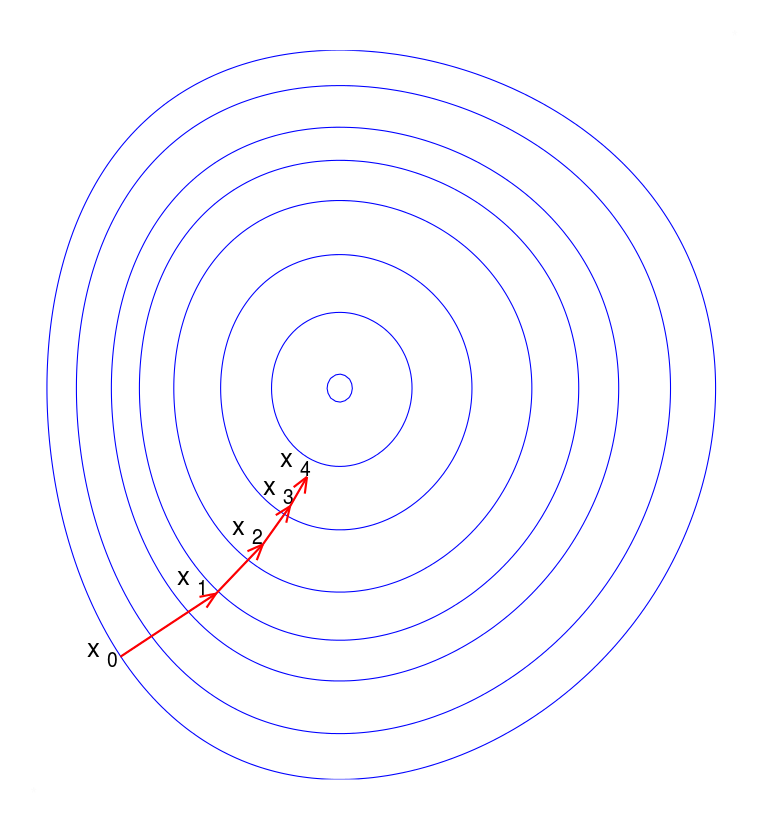
\includegraphics[width=0.3\textwidth]{img/sgd/level_sets.png}
\end{tabular}
\end{figure}
\end{frame}

%%%%%%%%%%%%%%%%%%%%%%%%%%%%%%%%%%%%%%%%%%%%%%%%%%%%%%%%%%%%%%%%%%

\begin{frame}{Visualizing Gradient Descent}
\begin{figure}
\begin{tabular}{c}
Gradient Descent for 1-d function $f(x)$.\\
  \animategraphics[loop,controls,width=0.9\textwidth]{1}{img/sgd/descent/descent-}{0}{7}
\end{tabular}
\end{figure}
\end{frame}


%%%%%%%%%%%%%%%%%%%%%%%%%%%%%%%%%%%%%%%%%%%%%%%%%%%%%%%%%%%%%%%%%%

\begin{frame}{Gradient Descent}
Turns out that if the function is \textbf{convex} gradient descent will converge to the \textbf{global minimum}. For \textbf{non-convex} functions, it may converge to \textbf{local minima}.
\begin{figure}
\begin{tabular}{cc}
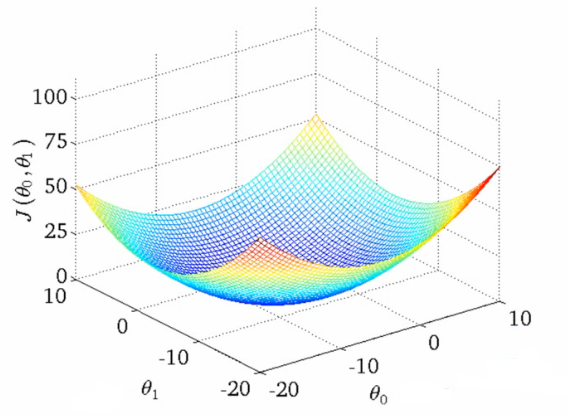
\includegraphics[width=0.4\textwidth]{img/sgd/convex_function.png} &
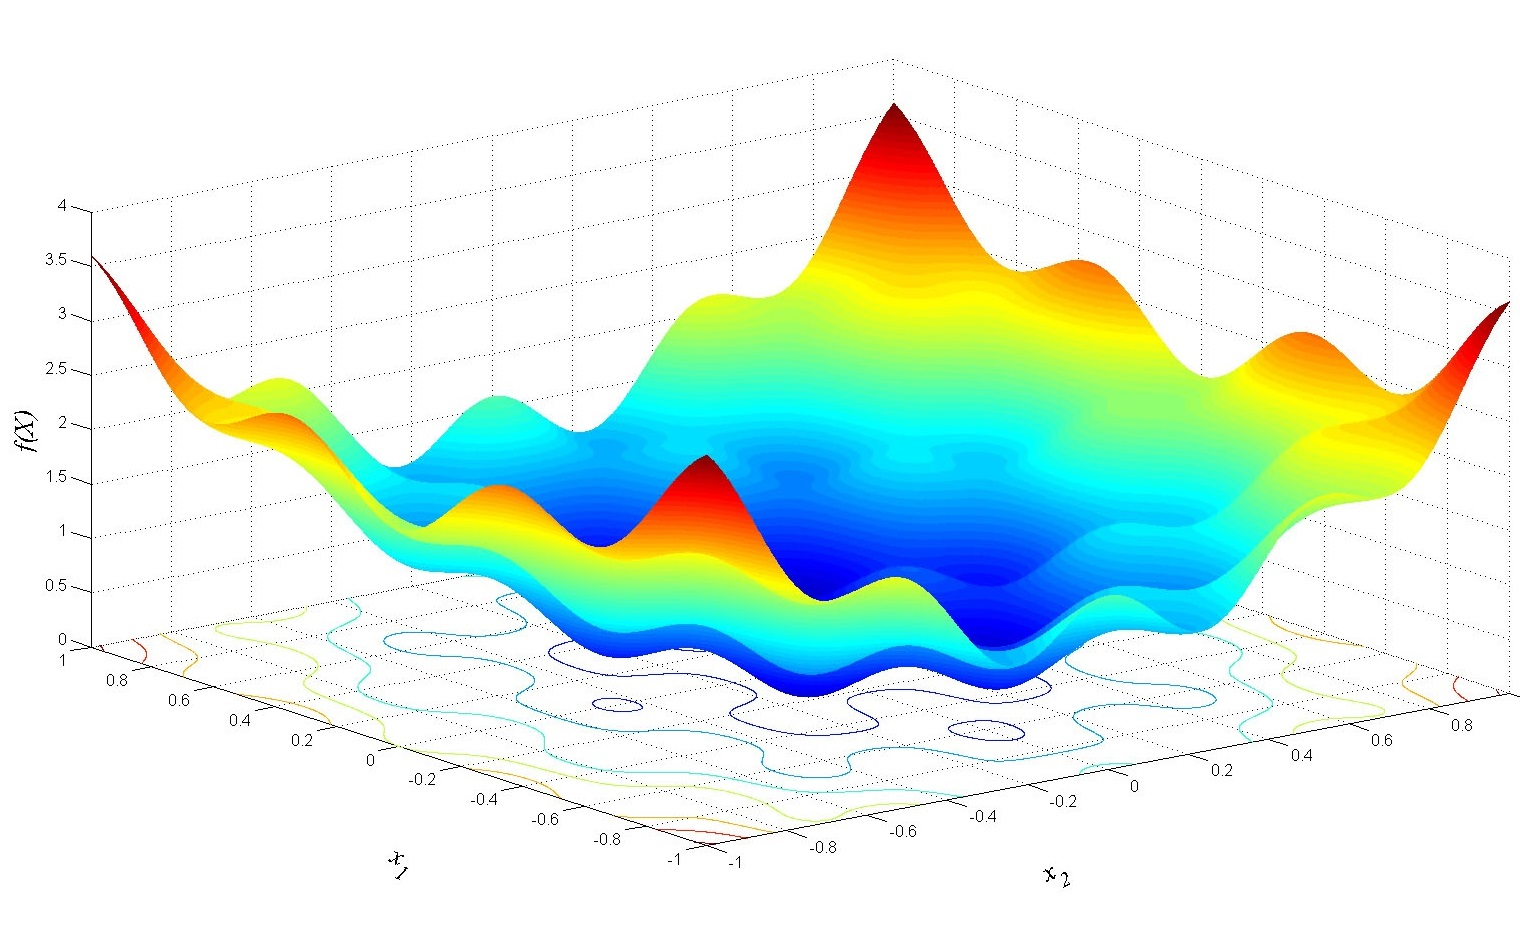
\includegraphics[width=0.4\textwidth]{img/sgd/non_convex_function.jpg}\\
Convex Function & Non-Convex Function
\end{tabular}
\end{figure}
\end{frame}

%%%%%%%%%%%%%%%%%%%%%%%%%%%%%%%%%%%%%%%%%%%%%%%%%%%%%%%%%%%%%%%%%%

\begin{frame}{Gradient Descent}
Gradient descent is often used in machine learning to \textbf{minimize a cost function}, often also called \textit{objective} or \textit{loss} function.\\
\vspace{0.5cm}
The cost function depends on the model's parameters and is a proxy to evaluate model's performance. Generally speaking, minimizing the cost equals to maximizing the effectiveness of the model.

\end{frame}

%%%%%%%%%%%%%%%%%%%%%%%%%%%%%%%%%%%%%%%%%%%%%%%%%%%%%%%%%%%%%%%%%%

\begin{frame}{Gradient Descent}
In practice, SGD

\end{frame}

%%%%%%%%%%%%%%%%%%%%%%%%%%%%%%%%%%%%%%%%%%%%%%%%%%%%%%%%%%%%%%%%%%

\begin{frame}{Gradient Descent}
Choosing the the right \textbf{learning rate} $\bm{\alpha}$ is essential to correctly proceed towards the minimum. A step \textit{too small} could lead to an extremely \textit{slow} convergence. If the step is \textit{too big} the optimizer could \textit{overshoot} the minimum or even \textit{diverge}. 
\begin{figure}
\begin{tabular}{ccc}
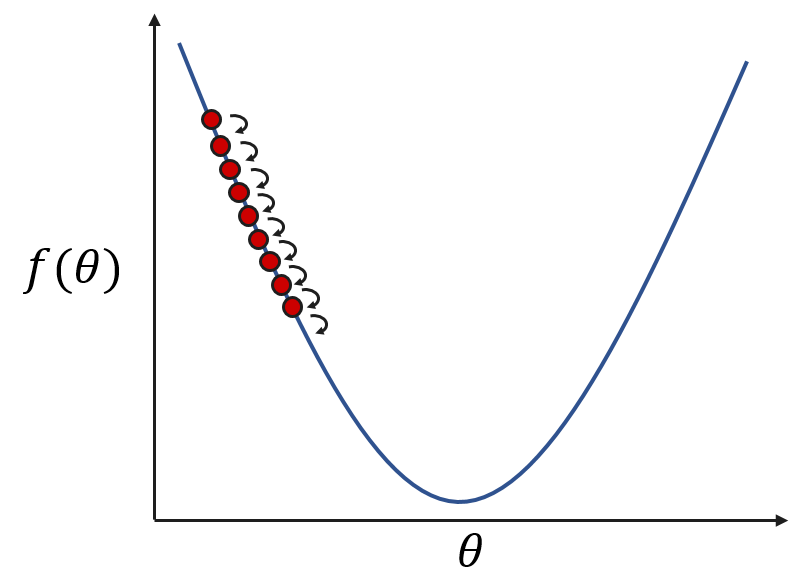
\includegraphics[width=0.35\textwidth]{img/sgd/lr_too_small.png} &
\quad &
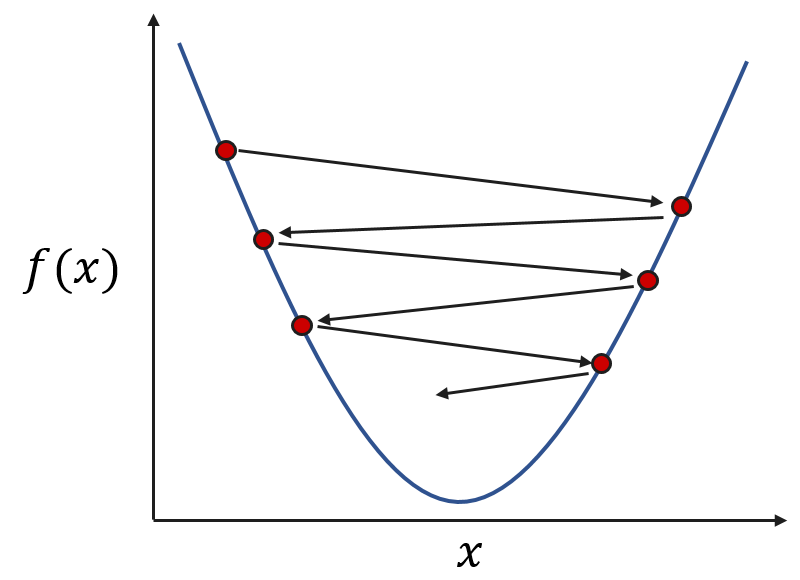
\includegraphics[width=0.35\textwidth]{img/sgd/lr_too_big.png}\\
Learning Rate too small & & Learning Rate too big
\end{tabular}
\end{figure}

\end{frame}

%%%%%%%%%%%%%%%%%%%%%%%%%%%%%%%%%%%%%%%%%%%%%%%%%%%%%%%%%%%%%%%%%%

\begin{frame}{Advanced Optimizers}
A number of different optimizer \cite{kingma2014adam,duchi2011adaptive,zeiler2012adadelta} are commonly used , but these are out of the scope of this short introduction.
\end{frame}



%%%%%%%%%%%%%%%%%%%%%%%%%%%%%%%%%%%%%%%%%%%%%%%%%%%%%%%%%%%%%%%%%%
%%%%%%%%%%%%%%%%%%%%%%%%%%%%%%%%%%%%%%%%%%%%%%%%%%%%%%%%%%%%%%%%%%
%%%%%%%%%%%%%%%%%%%%%%%%%%%%%%%%%%%%%%%%%%%%%%%%%%%%%%%%%%%%%%%%%%

\section{Credits}
\begin{frame}{Credits}
These slides heavily borrow from the following Stanford course:
\begin{itemize}
\item \url{http://cs231n.stanford.edu/}
\end{itemize}
if you want to deepen your knowledge of these concepts, I'd really suggest to start from here!\\
\vspace{0.2cm}
Also, nice convolution animations are taken from here:
\begin{itemize}
\item \url{https://github.com/vdumoulin/conv_arithmetic}
\end{itemize}
\end{frame}

%%%%%%%%%%%%%%%%%%%%%%%%%%%%%%%%%%%%%%%%%%%%%%%%%%%%%%%%%%%%%%%%%%
%%%%%%%%%%%%%%%%%%%%%%%%%%%%%%%%%%%%%%%%%%%%%%%%%%%%%%%%%%%%%%%%%%
%%%%%%%%%%%%%%%%%%%%%%%%%%%%%%%%%%%%%%%%%%%%%%%%%%%%%%%%%%%%%%%%%%

\section{References}

\begin{frame}[t, allowframebreaks]
\frametitle{References}
\bibliographystyle{abbrv}
\bibliography{bibliography}
\end{frame}
\end{document}